% Chapter 9

\chapter{Results on Radiative Corrections} % Chapter title

\label{ch:RC} % For referencing the chapter elsewhere, use \autoref{ch:name}

%----------------------------------------------------------------------------------------

The DJANGOH generator can be used in two ways: as a event generator inside a MC simulation or in a standalone way to compute radiative corrections. Here, DJANGOH is able to compute radiative correction factors in bins of ($x$,$y$,$z$), which was not possible with the previously used TERAD code.

\section{Inclusive radiative correction factors}\label{sec:RCF}

The calculation of the inclusive radiative correction factors is done by computing $\sigma_{Born}$ and $\sigma_{Born+\mathscr{O}(\alpha)}$. A correct way to obtain these factors is the following:
%
\begin{equation}
  \eta(x,y)=\frac{\sigma_{Born}(x,y)}{\sigma_{Born+\mathscr{O}(\alpha)}(x,y)}
  =\frac{\frac{\sigma_{Born,tot}*N_{Born}(x,y)}{N_{Born,tot}}}{\frac{\sigma_{Born+\mathscr{O}(\alpha),tot}*N_{Born+\mathscr{O}(\alpha)}(x,y)}{N_{Born+\mathscr{O}(\alpha),tot}}},
\end{equation}
%
where $\sigma_{Born+\mathscr{O}(\alpha),tot}$ and $\sigma_{Born,tot}$ are the integrated Born+$\mathscr{O}(\alpha)$ and Born DIS cross-section over the imposed kinematic boundaries respectively, $N_{Born+\mathscr{O}(\alpha),tot}$ and $N_{Born,tot}$ are the total number of DIS events generated with Born+$\mathscr{O}(\alpha)$ and Born DIS cross-section respectively, and $N_{Born+\mathscr{O}(\alpha),tot}(x,y)$ and $N_{Born,tot}(x,y)$ are the DIS events generated in a given $(x,y)$ bin with Born+$\mathscr{O}(\alpha)$ and Born DIS cross-section respectively. The results that are presented below are obtained with the TERAD $F_{2}$ and R parametrizations, which describes accurately the behaviour of $F_{2}$ at low $Q^{2}$ \cite{BPnote}:

\begin{itemize}
\item $F^{p}_{2}(x,Q2)$ for $Q^2 > 0.2$ GeV$^2$ and $0.000035 < x < 0.85$, as obtained from a fit to the
world proton (and deuteron) data made by the SMC \cite{SMC}.
\item For $Q^2 < 0.2$ GeV$^2$, a phenomenological model of Badelek and Kwiecinski \cite{BK}, valid at $10^{-5} < x < 0.1$
and $0 < Q^2 < 1000$ GeV$^2$.
\item $R(x, Q^2)$ as parameterised by SLAC (newer version, called R1998 \cite{R1998}), valid for $Q^2 > 0.5$ GeV$^2$, extended
to lower values of $Q^2$, including the $R \simeq Q^2$ behaviour at $Q^2 = 0$.
\end{itemize}

All first order QED corrections are included except for quark line radiation. The reason why these corrections are not included is that these corrections are negligible except at large $x \geq 0.5$ and $Q^{2} \geq 10^3$ (GeV/$c$)$^2$, where the corrections reach the magnitude of barely one percent (see Fig.~\ref{fig:quarkline}). In addition, these corrections are often not subtracted inside the parametrization, thus they are already taken into account in the parametrization \cite{HubertF2Rad}. In contrast they are considered in TERAD in a QPM-like approach.

\begin{figure}[htb]
\centerline{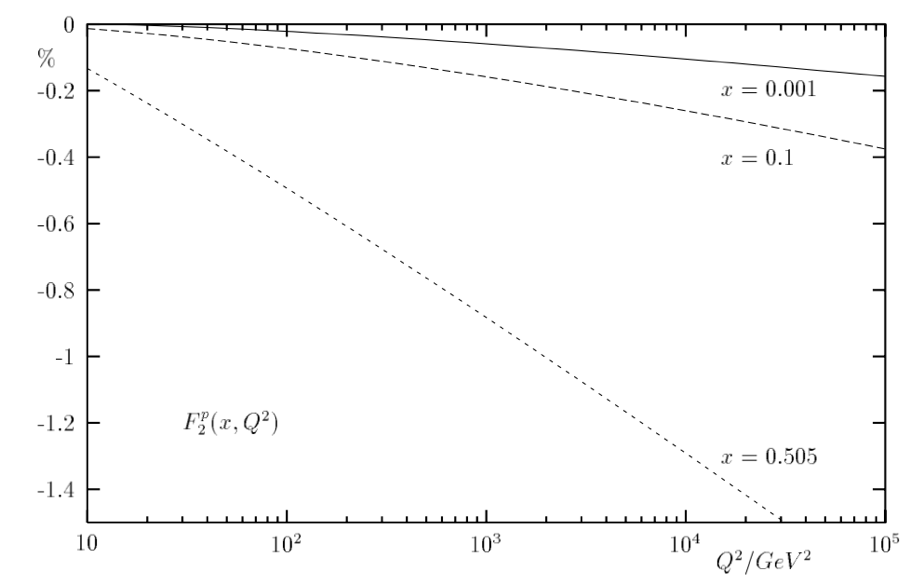
\epsfig{file=gfx/quarkline.png,width=12cm}}
\caption{$Q^2$ dependence of the quarkonic QED corrections (in percent) to the structure function $F^p_2$ for deep inelastic
lepton-proton scattering at $x=0.001$, $x=0.1$ and $x=0.505$. Figure taken from \cite{HubertF2Rad}.}\label{fig:quarkline}
\end{figure}

%----------------------------------------------------------------------------------------

\section{Comparison between DJANGOH and TERAD}

DJANGOH results for inclusive radiative corrections are compared with TERAD \cite{TERAD}. The two programs are using the same set of $F^{p}_{2}$ and $R$. This are the only inputs (apart from the process input ie. $\mu p$ scattering at 160 GeV muon energy) that need to be identical so that the comparison is relevant. One thing to be noted is that TERAD is using in addition $\mathscr{O}(\alpha^2)$ corrections. They should have an impact on the cross-section of TERAD, but are negligible.

The first check for consistency done in Fig.~\ref{fig:BRy} is to compare the $\sigma_{Born}$ of both programs. Using the same input information on $F^{p}_{2}(x,Q2)$ and $R(x, Q^2)$ does not guarantee that $\sigma_{Born}$ for both program, called $\sigma^{D}_{Born}$ and $\sigma^{T}_{Born}$, is the same, even if the structure functions should define the Born cross-section unambiguously. The reason is that in TERAD, $\sigma^{T}_{Born}$ is computed without constants like $\pi$, $M_{proton}$, $\alpha$, etc. and its functional form is unknown, unlike in DJANGOH. This means that the ratio $r=\frac{\sigma^{D}_{Born}}{\sigma^{T}_{Born}}$ may slightly differ from 1 but must be constant as a function of $x$ and $y$.

\begin{figure}[!htb]
\centerline{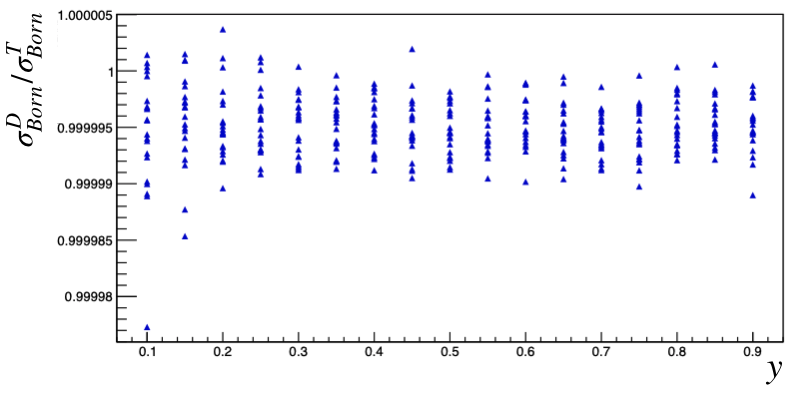
\epsfig{file=gfx/BRy.png,width=14cm}}
\caption{Ratio of the Born cross-sections calculated with DJANGOH and TERAD, for the same $F_2$ and $R$ parametrizations, as a function of $y$ at different values of $x$ (staggered points at fixed $y$)}\label{fig:BRy}
\end{figure}

The radiative correction factors $\eta(x,y)$ for DJANGOH ($\eta_D$) and TERAD ($\eta_T$) are compared in Fig.~\ref{fig:RCy}. The relative difference shows that the two programs differ at most $3$\% in the region of lowest $x$ and highest $y$. This results is extremely good, knowing that DJANGOH and TERAD are not using the same renormalization scheme.


\begin{figure}[htb]
\centerline{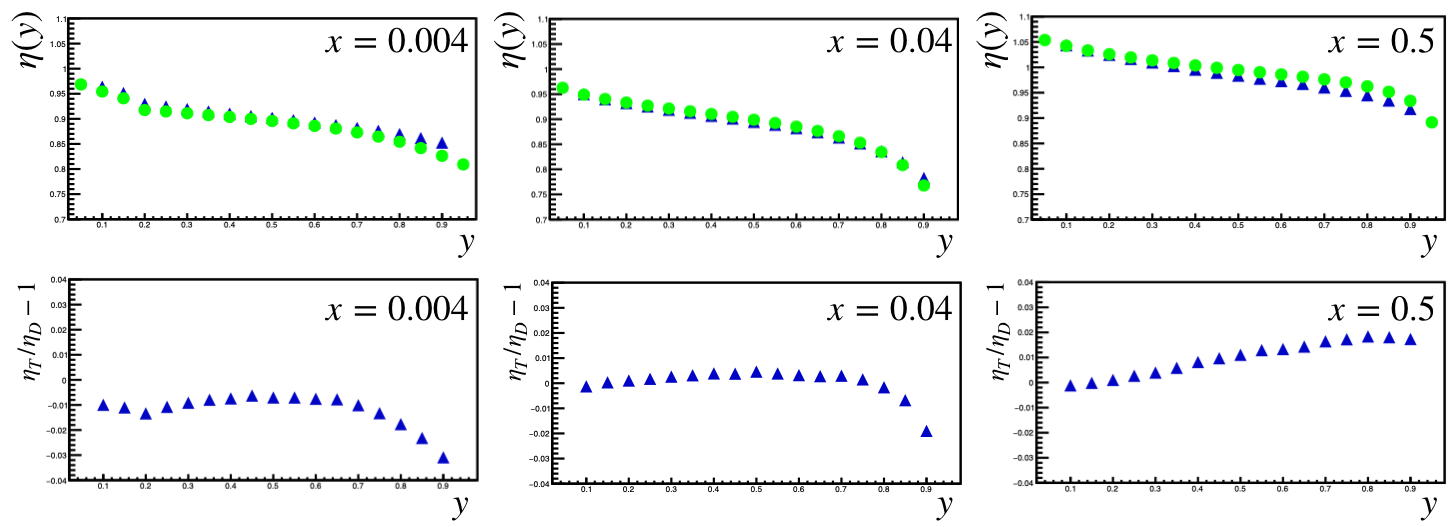
\epsfig{file=gfx/RCy.png,width=14cm}}
\caption{In top panels, comparison of radiative corrections factor $\eta(y)$ for fixed values of $x$, computed for proton target at 160 GeV and with the same $F^p_2$ and $R$ parametrizations. Green dots mark results of TERAD, blue triangles the results of DJANGOH. In bottom panels, relative difference of radiative corrections factors $(\eta_T/\eta_D)-1$ as a function of $y$ for fixed values of $x$}\label{fig:RCy}
\end{figure}


%----------------------------------------------------------------------------------------

\section{Radiative correction factors: Effect on Multiplicities}\label{sec:RCFMult}

The calculation of the radiative correction factors for the multiplicities can be done by computing $M^{h}_{Born}$, multiplicities obtained without radiative corrections, and $M^{h}_{Born+\mathscr{O}(\alpha)}$, multiplicities obtained with radiative corrections. The factors are given as:
%
\begin{equation}
  \begin{split}
    \eta^{h}(x,y,z)=\frac{M^{h}_{Born}(x,y,z)}{M^{h}_{Born+\mathscr{O}(\alpha)}(x,y,z)} \\
     = \frac{N^{h}_{Born}(x,y,z)/N^{DIS}_{Born}(x,y)}{N^{h}_{Born+\mathscr{O}(\alpha)}(x,y,z)/N^{DIS}_{Born+\mathscr{O}(\alpha)}(x,y)}
  \end{split}
\end{equation}
%
where $N^h$ is the number of hadrons and $N^{DIS}$ the number of DIS events.

For the calculation of the radiative correction factors the cuts from the SIDIS analysis for the selection of DIS events and hadrons are used (see Chapter~\ref{ch:raw} for further details). The kinematical cuts used are:

\begin{itemize}
\item $0.004 \leq x \leq 0.4, x \in \{.004,.01,.02,.03,.04,.06,.1,.14,.18,.4\}$
\item $0.1 \leq y \leq 0.7, y \in \{.1,.15,.2,.3,.5,.\}$
\item $12 \leq p_h \leq 40$ GeV/$c$
\end{itemize}

Fig.~\ref{fig:hadz_ratio} exhibits the semi-inclusive radiative correction factor $\eta^{h}(x,y,z)$. This factor goes from $2$\% correction at high $x$ to $20$\% correction at high $z$ and high $y$. This dependence on $y$ and $z$ is expected (for instance if a hadron has a high $z$ in a non-radiative event, consider the same event but with the radiation of a real photon, $\nu_{lep}$ will remain the same but the hadron will have in reality less energy available from the virtual photon, thus having $z_{had} \leq z_{lep}$, leading to less events in the high $z$ region for the multiplicities obtained with radiative correction). The results are obtained at generator level but they should be the same if one uses reconstructed MC to compute them. However as a huge number of events is needed to obtain such results (about 1 billion events), computing them would require an amount of reconstructed MC that largely overshoot our biggest MC productions.

\begin{figure}[!htb]
\centerline{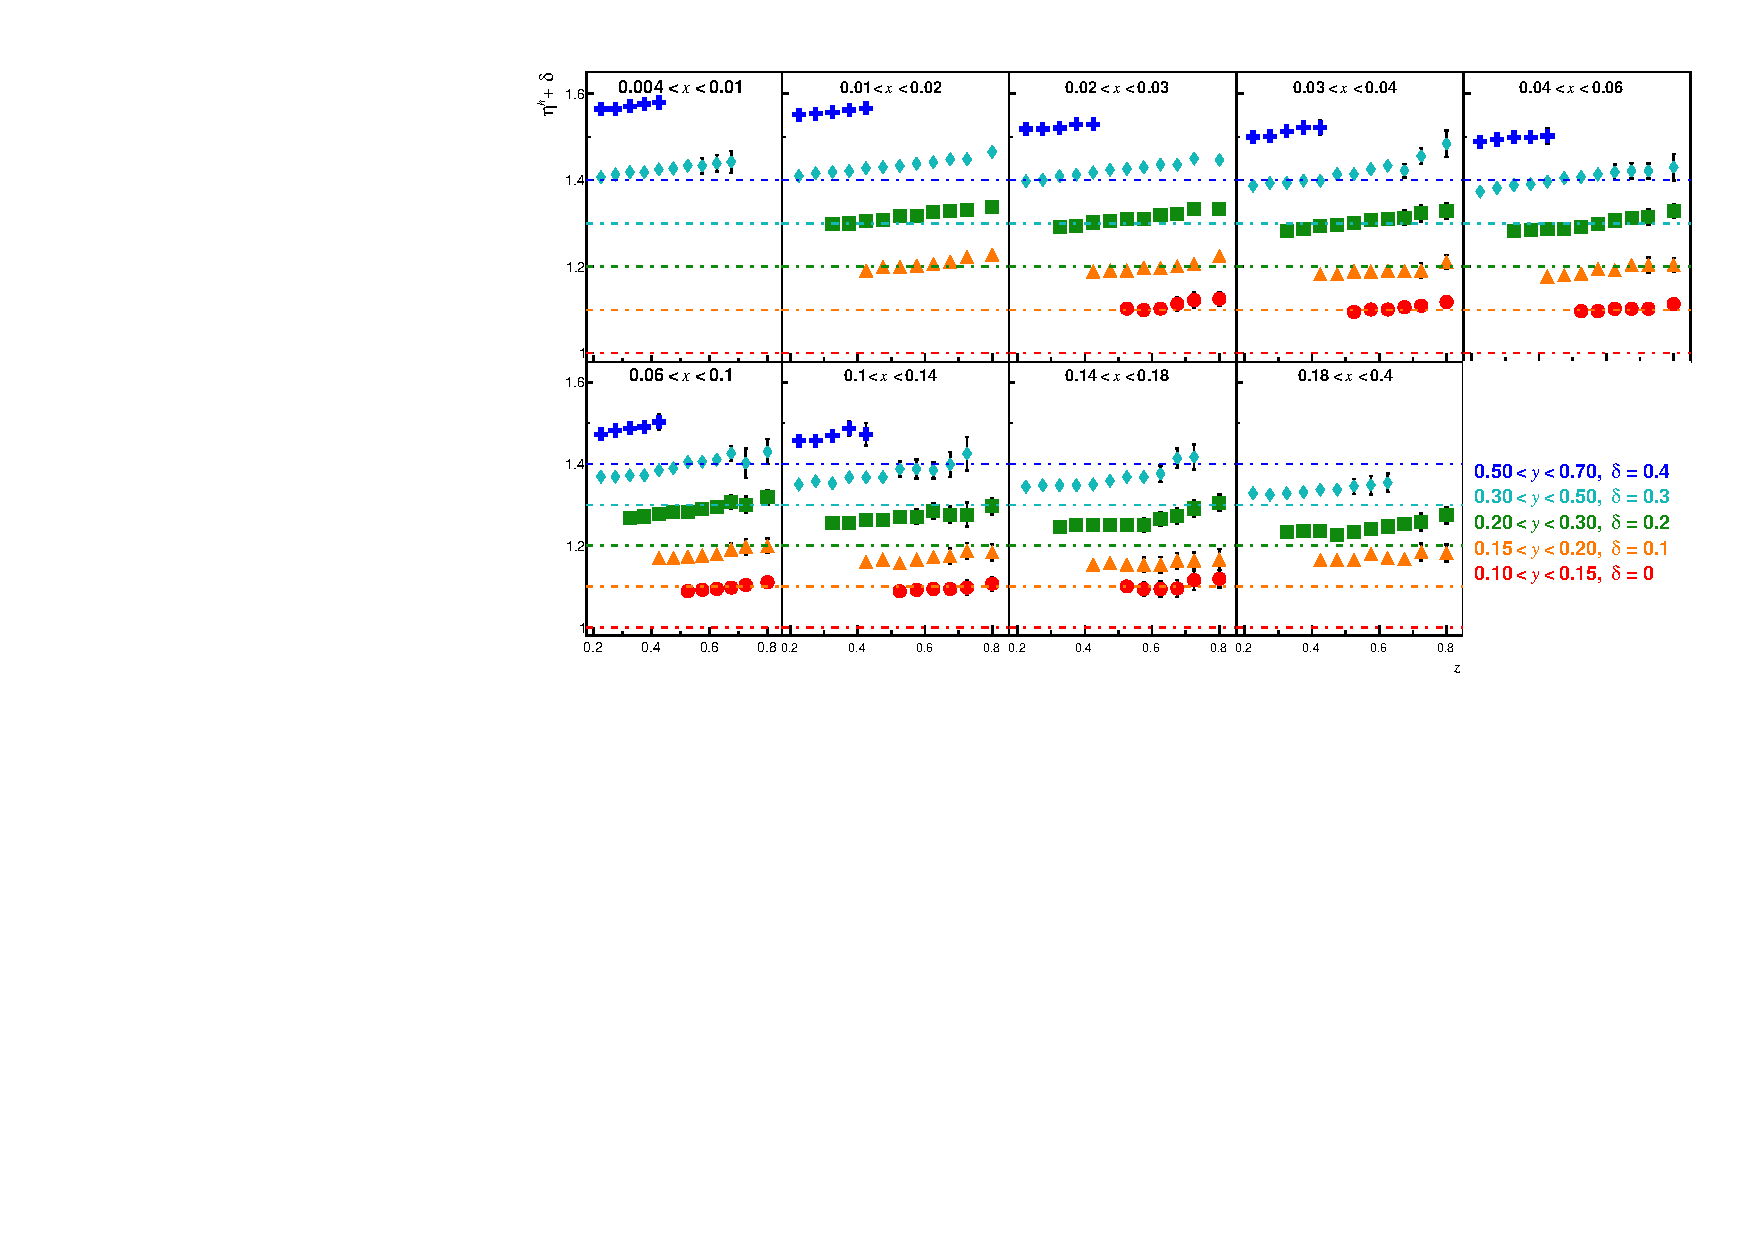
\epsfig{file=gfx/hadron_ratio.pdf,width=16cm}}
\caption{$\eta^{h}(x,y,z)$, positive hadrons in full points, negative in open points, in bins of $x$, staggered with $y$ and versus $z$. The corrections go from $2$\% at high $x$ to $20$\% at high $z$ and high $y$.}\label{fig:hadz_ratio}
\end{figure}

%----------------------------------------------------------------------------------------

\section{Summary}

The DJANGOH event generator with radiative events is a way to access radiative correction factor in a three dimensional ($x$,$y$,$z$) binning, like in the multiplicity analysis. This is the first time that such corrections are available for the COMPASS data. The size of the correction, going from $2$ to $20$\% is within the expectations. Moreover, this correction can directly be applied on the multiplicities. When compared with TERAD computation on the inclusive corrections, the results of DJANGOH are shown to be compatible within $3$\%, a really good result knowing that DJANGOH and TERAD are not using the same renormalization scheme. A four-dimensional ($x$,$y$,$z$,$p_T$) binning could also be done but it would need way more statistics that what was used for the three dimensional ($x$,$y$,$z$) binning.
